% ── Section III: Method ──────────────────────────────────────────────
% Conference budget: ~2 pages. Math matches the implementation exactly:
%   C1: code/models/context_estimator.py + adaptive_controller.py
%   C2: code/models/motorcycle_motion_model.py
%   C3: code/models/track_reliability.py
% ─────────────────────────────────────────────────────────────────────

\section{Method}
\label{sec:method}

\subsection{System Overview}
\label{subsec:overview}

Fig.~\ref{fig:pipeline} shows the pipeline.
Each frame first passes through the \emph{context estimator} (C1),
which summarizes the current traffic state from the frame and the
tracker's recent history; the \emph{adaptive parameter controller} (C1)
maps that state to a detector confidence threshold, a lost-track buffer
length, and a motion-model selection.
YOLO11~\cite{Khanam2024_yolo11} detections then enter a modified
ByteTrack~\cite{Zhang2022_bytetrack} in which motorcycle tracks are
predicted by a CTRV extended Kalman filter and all other classes by the
original linear filter (C2), and in which the filter's own uncertainty
re-opens association for tracks that IoU alone would lose; ByteTrack's
two-stage matching itself is unchanged.
Finally, every confirmed track receives a \emph{reliability score}
(C3), and two thresholds split the output: high-reliability tracks feed
the accident-detection branch (EfficientNet-B0
severity classifier~\cite{Tan2019_efficientnet} and operator alerts),
while a more permissive threshold passes tracks to the observation
builder of a MAPPO-based~\cite{Yu2022_mappo} signal controller.

\begin{figure}[t]
  \centering
  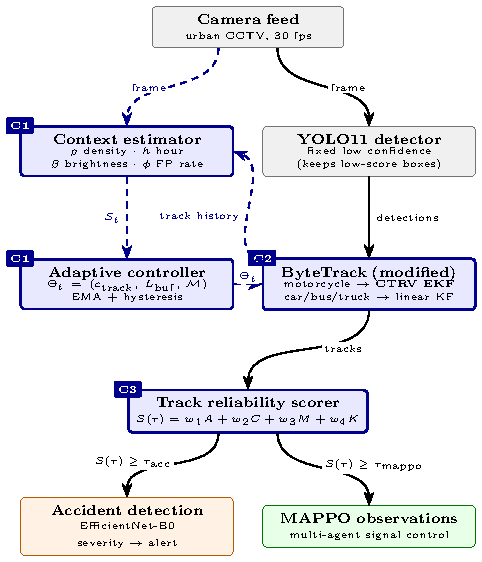
\includegraphics[width=0.96\linewidth]{figures/fig1_pipeline_overview.pdf}
  \caption{Context-aware adaptive perception pipeline.
           Solid arrows carry data; dashed arrows carry context and
           control signals.
           The three proposed modules are tagged C1--C3 (blue);
           detector and association logic are standard.
           One reliability score $S(\tau)$ feeds both downstream tasks
           through two thresholds
           ($\tau_{\mathrm{acc}} > \tau_{\mathrm{mappo}}$).}
  \label{fig:pipeline}
\end{figure}

\subsection{C1: Context Estimator and Adaptive Parameter Controller}
\label{subsec:c1}

Fixed operating points are tuned for one regime and fail in others: a
threshold chosen for free-flowing daytime traffic drops detections in
dense scenes and hallucinates them at night.
C1 closes this loop with a deliberately lightweight design --- four
scalar signals and a rule table --- so that adaptation itself adds no
perceptible latency.

\paragraph{Context signals}
At frame $t$ the estimator computes the traffic state
\begin{equation}
  \mathcal{S}_t = \left(\rho_t,\; h_t,\; \beta_t,\; \phi_t\right),
  \label{eq:state}
\end{equation}
where $\rho_t$ is the number of active tracks (density), $h_t \in
\{0,\dots,23\}$ the hour of day, $\beta_t \in [0,255]$ the mean
grayscale intensity (lighting proxy), and
$\phi_t = |\{\tau : \mathrm{age}(\tau) < 3\}| / |\mathcal{T}_t|$
the fraction of short-lived tracks among active tracks
$\mathcal{T}_t$, an online proxy for the current false-positive rate.
Density and brightness are smoothed with an exponential moving average,
$\tilde{s}_t = \alpha s_t + (1-\alpha)\,\tilde{s}_{t-1}$ with
$\alpha = 0.1$, so single-frame flicker (headlight glare, a dropped
detection burst) does not thrash the controller.

\paragraph{Parameter mapping}
The controller classifies $\mathcal{S}_t$ into one of three conditions
with priority \textsc{night} $>$ \textsc{dense-peak} $>$
\textsc{default}: \textsc{night} if $\beta_t < \beta_{\min}$, and
\textsc{dense-peak} if $\rho_t \geq \rho_{\min}$ during peak hours.
Each condition indexes one row of Table~\ref{tab:param_table},
producing the parameter set
$\Theta_t = (c_{\mathrm{track}}, L_{\mathrm{buf}}, \mathcal{M})$:
the tracker's confirmation threshold, the lost-track buffer length, and
the motion-model selector.
Following ByteTrack's two-stage association, the detector itself always
runs at a low fixed confidence so that low-score boxes remain available
for second-stage association; $c_{\mathrm{track}}$ instead gates track
confirmation.
In dense scenes the buffer is lengthened and CTRV enabled, favoring
recall through occlusions; at night the threshold rises and the buffer
shrinks, suppressing low-contrast false positives.
The \textsc{night} row keeps the linear motion model --- its
conservatism is expressed entirely through the stricter threshold and
shorter buffer.

\begin{table}[t]
  \centering
  \caption{Adaptive parameter table. \textsc{dense-peak} is calibrated
           against ground truth (Sec.~\ref{subsec:ablation_results});
           the other two rows await footage that exercises them.}
  \label{tab:param_table}
  \begin{tabular}{lcccl}
    \toprule
    Condition & $c_{\mathrm{track}}$ & $L_{\mathrm{buf}}$ (frames)
              & $\mathcal{M}$ & source \\
    \midrule
    \textsc{dense-peak} & 0.50 & 30 & CTRV (motorcycle) & calibrated \\
    \textsc{night}      & 0.55 & 20 & linear & initial \\
    \textsc{default}    & 0.45 & 30 & linear & initial \\
    \bottomrule
  \end{tabular}
\end{table}

The calibrated \textsc{dense-peak} row inverts the design intuition that
motivated it.
We expected dense scenes to want a \emph{lower} confirmation threshold,
trading precision for recall through occlusion; measured against ground
truth the opposite holds, and $c_{\mathrm{track}} = 0.50$ --- stricter
than \textsc{default} --- is optimal.
At $\sim$47 vehicles per frame the additional weak detections admitted by
a low threshold generate far more false positives than they recover true
objects.
We report this because it is the kind of assumption that a fixed-threshold
baseline never has to confront, and because it bears directly on whether
context adaptation helps at all (Sec.~\ref{subsec:ablation_results}).

\paragraph{Hysteresis}
Raw threshold rules oscillate when a signal hovers near a boundary.
A condition therefore becomes active only after being observed for
$N_h = 15$ consecutive frames ($0.5$\,s at 30\,fps); until then the
controller holds the previous parameter set.
This stabilizes the tracker against boundary noise while still
reacting within a second to genuine regime changes.

\subsection{C2: Class-Conditioned CTRV Motion Model}
\label{subsec:c2}

ByteTrack's Kalman filter assumes constant velocity in the image
plane, which is adequate for cars but not for motorcycles: a weaving
motorcycle turns \emph{continuously}, so during an occlusion the linear
filter coasts straight while the true object follows an arc, and the
reappearing detection falls outside the association gate.
We therefore condition the motion model on the detected class:
motorcycle tracks receive a CTRV~\cite{Schubert2008_ctrv} extended
Kalman filter (EKF); cars, buses, and trucks keep the original linear
filter.
Association is untouched --- both filters expose the same
predict/update interface and output a predicted box for IoU matching.

\paragraph{Process model}
The CTRV state is
$\mathbf{x} = [\,p_x,\; p_y,\; v,\; \theta,\; \omega\,]^\top$:
image-plane position, speed, heading, and turn rate.
With time step $\Delta t$ (one frame), the discretized process model is
\begin{align}
  p_{x,k+1}    &= p_{x,k} + v_k \cos\theta_k \,\Delta t, \label{eq:ctrv_x}\\
  p_{y,k+1}    &= p_{y,k} + v_k \sin\theta_k \,\Delta t, \label{eq:ctrv_y}\\
  \theta_{k+1} &= \theta_k + \omega_k \,\Delta t,        \label{eq:ctrv_theta}
\end{align}
with $v$ and $\omega$ constant across the step.
We use this Euler form rather than the exact arc integral, which
removes the $\omega \to 0$ singularity of the closed-form CTRV
equations; at 30\,fps the per-step discretization error is negligible.
A nonzero $\omega$ estimate makes the predicted position rotate its
heading each step --- the filter coasts \emph{along the arc} through
occlusions, which is exactly the regime where the linear model fails.

\paragraph{EKF prediction and update}
The process model is nonlinear in $\theta$, so prediction propagates
the covariance with the Jacobian
$\mathbf{F}_k = \partial f / \partial \mathbf{x}\,|_{\mathbf{x}_k}$,
whose nontrivial entries are
$\partial p_x / \partial v = \cos\theta\,\Delta t$,
$\partial p_x / \partial \theta = -v\sin\theta\,\Delta t$,
$\partial p_y / \partial v = \sin\theta\,\Delta t$,
$\partial p_y / \partial \theta = v\cos\theta\,\Delta t$, and
$\partial \theta / \partial \omega = \Delta t$:
\begin{equation}
  \mathbf{P}_{k+1|k} = \mathbf{F}_k \mathbf{P}_k \mathbf{F}_k^\top
                       + \mathbf{Q}.
\end{equation}
The measurement is the detection-box center,
$\mathbf{z} = [p_x, p_y]^\top = \mathbf{H}\mathbf{x}$ with linear
$\mathbf{H}$, so the update is a standard Kalman step; we use the
Joseph-form covariance update for numerical symmetry over long
sequences.
Box width and height are taken from the last matched detection and
held constant while the track is lost, since association only requires
a well-placed box.

\paragraph{Heading bootstrap}
Speed and heading are unobservable from a single detection.
Rather than letting the EKF infer them slowly through the position
cross-covariances, we initialize $v$ and $\theta$ directly from the
displacement between the first two detections (when it exceeds a small
noise floor), resetting the corresponding covariance entries.
This one-step bootstrap removes the $\sim$10-frame convergence delay
that would otherwise erase CTRV's advantage on short tracks.

\paragraph{Uncertainty-gated re-association}
A better prediction is only useful if association can act on it.
IoU matching fails exactly when the motion model matters most: after a
long occlusion the predicted and reappearing boxes may not overlap at
all, giving zero IoU and no possibility of a match at any threshold.
The EKF, however, also reports \emph{how uncertain} that prediction is.
For a lost motorcycle track we form the innovation covariance
$\mathbf{S} = \mathbf{H}\mathbf{P}\mathbf{H}^\top + \mathbf{R}$ and
admit a same-class detection $\mathbf{z}$ when its squared Mahalanobis
distance falls inside the $95\%$ ellipse,
\begin{equation}
  d^2 = (\mathbf{z} - \mathbf{H}\mathbf{x})^\top \mathbf{S}^{-1}
        (\mathbf{z} - \mathbf{H}\mathbf{x}) < \chi^2_{0.95,2} = 5.991 .
  \label{eq:gate}
\end{equation}
Admitted pairs do not win outright; they enter the cost matrix at
\begin{equation}
  c_{\mathrm{gate}} = c_0 + (1 - c_0)\, d^2 / \chi^2_{0.95,2},
  \qquad c_0 = 0.5,
  \label{eq:gate_cost}
\end{equation}
so rescued costs lie in $[0.5, 1)$ and always lose to a genuine IoU
overlap.
The gate therefore never overrides ordinary association --- it only
makes a match \emph{possible} where IoU alone offers none.
Tracked (non-lost) and linear-filter tracks are untouched.

\paragraph{Confidence-scaled measurement noise}
The gate's usefulness depends on $\mathbf{S}$ being both tight and
correctly centered, which in turn depends on how much the filter trusts
its detections.
Following StrongSORT~\cite{Du2023_strongsort}, we scale the measurement
noise by detection confidence $s$,
\begin{equation}
  \mathbf{R}_{\mathrm{eff}} = \mathbf{R}\,
    \mathrm{clip}(1 - s,\; 0.05,\; 1),
  \label{eq:nsa}
\end{equation}
with the floor preventing a near-perfect detection from making
$\mathbf{R}$ singular.
Confident detections pull the state onto the measurement; weak ones
leave the motion model in charge.

\paragraph{One mechanism, not three}
These components are not independent improvements to be credited
separately, and Sec.~\ref{subsec:ablation_results} shows the gate
\emph{alone} makes identity worse.
The reason is that Eqs.~\eqref{eq:gate} and~\eqref{eq:nsa} act on the
same quantity.
With an untightened $\mathbf{R}$ the filter over-smooths, so the
predicted center lags a weaving motorcycle while $\mathbf{P}$ --- and
hence $\mathbf{S}$ --- grows: the admission ellipse of
Eq.~\eqref{eq:gate} becomes simultaneously wide and mis-centered, and
the detections it admits are frequently the wrong ones.
Rescues then transfer identities between neighboring motorcycles, which
in dense traffic is worse than not rescuing at all.
Eq.~\eqref{eq:nsa} is what makes the ellipse trustworthy; the gate is
what makes it useful.
We therefore report C2 as a single class-conditioned motion mechanism
and ablate its parts only to expose this interaction.

\begin{algorithm}[t]
  \caption{Class-conditioned prediction and association}
  \label{alg:motion_model}
  \begin{algorithmic}[1]
    \For{each active track $\tau$}
      \If{$\mathrm{class}(\tau) = \texttt{motorcycle}$}
        \State $\hat{\mathbf{b}}_\tau \gets$ CTRV-EKF predict
               (Eqs.~\ref{eq:ctrv_x}--\ref{eq:ctrv_theta})
      \Else
        \State $\hat{\mathbf{b}}_\tau \gets$ linear Kalman predict
               (original ByteTrack)
      \EndIf
    \EndFor
    \State $\mathbf{C} \gets$ IoU cost on $\{\hat{\mathbf{b}}_\tau\}$
    \For{each \emph{lost} CTRV track $\tau$ and same-class detection
         $\mathbf{z}$}
      \If{$d^2(\tau, \mathbf{z}) < \chi^2_{0.95,2}$}
        \State $C_{\tau,\mathbf{z}} \gets
               \min(C_{\tau,\mathbf{z}},\, c_{\mathrm{gate}})$
               (Eq.~\ref{eq:gate_cost})
      \EndIf
    \EndFor
    \State run unchanged ByteTrack two-stage association on $\mathbf{C}$
    \State update matched CTRV tracks with $\mathbf{R}_{\mathrm{eff}}$
           (Eq.~\ref{eq:nsa})
  \end{algorithmic}
\end{algorithm}

\subsection{C3: Dual-Task Track Reliability Score}
\label{subsec:c3}

The two downstream consumers impose conflicting operating points.
Accident alerting must be precise --- every alert interrupts an
operator --- so it should only trust well-established tracks.
The MAPPO observation builder must be complete --- a dropped vehicle is
a hole in the controller's state --- so it should tolerate
medium-quality tracks.
Instead of tuning two separate pipelines, C3 computes one scalar
reliability per track and applies two thresholds.

\paragraph{Score}
For track $\tau$,
\begin{equation}
  S(\tau) = w_1 A(\tau) + w_2 C(\tau) + w_3 M(\tau) + w_4 K(\tau)
          + w_5 D(\tau),
  \label{eq:reliability}
\end{equation}
with $\sum_i w_i = 1$ and, over a sliding window of $N{=}10$ frames:
$A(\tau) = \min(\mathrm{age}(\tau)/T_{\max},\,1)$ the normalized track
age ($T_{\max} = 30$ frames);
$C(\tau)$ the detection hit rate (fraction of window frames with a
matched detection);
$M(\tau)$ the mean IoU between the track's predicted and matched
detected boxes;
$K(\tau)$ the fraction of window frames whose detected class equals the
track's modal class; and
$D(\tau)$ the mean confidence of the matched detections.
We use \emph{mean} predicted-vs-detected IoU for motion smoothness
rather than inverse IoU variance: a consistently badly predicted track
has low variance but is not reliable, whereas mean IoU is monotone in
prediction quality and already penalizes erratic motion.
The detection-confidence term $D$ closes a blind spot we observed on
real footage: ByteTrack's second association stage can sustain a
``ghost'' track indefinitely on sub-threshold detections (shadows, road
texture), so the track matches \emph{every} frame and $A$, $C$, $K$ are
all perfect --- only the matched detection score separates it from a
real object.
Weights are set to $(w_1,\dots,w_5) = (0.1, 0.2, 0.25, 0.15, 0.3)$
% TODO: replace with grid-searched values + sensitivity note (Sec. V)
and calibrated on the training split.

\paragraph{Cold start}
With fewer than three window samples, the history-based components
return a neutral $0.5$; combined with the near-zero age term this keeps
brand-new tracks below the accident threshold \emph{by construction} ---
short-lived spurious tracks, the dominant false-alert source, are
suppressed without any dedicated rule.

\paragraph{Dual thresholds}
The accident branch consumes tracks with
$S(\tau) \geq \tau_{\mathrm{acc}}$ (precision-first) and the MAPPO
observation builder consumes tracks with
$S(\tau) \geq \tau_{\mathrm{mappo}}$, where
$\tau_{\mathrm{mappo}} < \tau_{\mathrm{acc}}$ (recall-first);
we use $\tau_{\mathrm{acc}} = 0.7$ and $\tau_{\mathrm{mappo}} = 0.4$.
A single scoring pass thus serves both tasks without retuning either.

On our data $\tau_{\mathrm{mappo}}$ sits below the lowest score any track
attains, so the MAPPO branch is pass-through: maximal recall, which is
the intended behavior for that consumer, but it means C3 contributes
nothing measurable to the tracking metrics.
Sweeping $\tau_{\mathrm{mappo}}$ upward is strictly worse
(Sec.~\ref{subsec:ablation_results}), and we report in
Sec.~\ref{subsec:c3_limits} why this follows from the score's
discriminative power rather than from the choice of threshold.
The precision branch is where the dual-task claim would be tested, and
our footage contains no accidents; we therefore present C3 as a
formulation with a characterized failure mode, not as a validated
contribution.
